
\begin{frame}
    \frametitle{Historie}
    \begin{itemize}
        \item Vynálezci: Wilbert L. Gore a Robert W. Gore 
        \item Rok: 1969
        \item Vynález víceméně náhodou při experimentování s materiálem PTFE
    \end{itemize}
\end{frame}

\section{Struktura materiálu}

\begin{frame}
    \frametitle{Co se skrývá pod názvem Gore-Tex \textregistered }
    \begin{itemize}
        \item Expandovaný polytetrafluorethylen (všeobecně znám pod obchodním názvem Teflon\textregistered)
            % Takže natažená pánvička?
        \item Zkratka (anglická): ePTFE %TODO: zkontrolovat je jen anglická?
        \item Membrána se z PTFE získá rychlým trhem po zahřátí materiálu (odtud expandovaný, natažený)

    \end{itemize}

    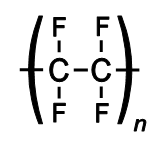
\includegraphics[width=0.2\textwidth]{Teflon_structure.PNG}

    \zdroj{GPL, https://commons.wikimedia.org/w/index.php?curid=839743}

\end{frame}

\begin{frame}
    \frametitle{Struktura}
    \begin{figure}
        \begin{center}
            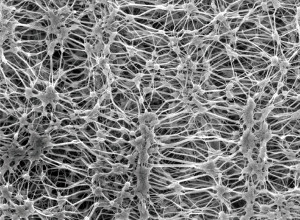
\includegraphics[width=200pt]{membrane_microscopy_small.jpg}
            \caption{Membrána na snímku z elektronového mikroskopu}
            \label{fig:membrana}
        \end{center}
    \end{figure}
    \zdroj{http://www.evo.com/waterproof-ratings-and-breathability-guide.aspx}
\end{frame}

\begin{frame}
    \frametitle{Struktura}
    \begin{itemize}
            \item 1.4 miliardy pórů na centimetr čtvereční: \\
                $ \sqrt{10^{-4}/1.4\cdot10^{9}} = 267 nm $
            \item Jeden pór je 700x větší než molekula páry: \\
                $ 0.4nm \cdot 700 = 280 nm $ \\
                Kde 0.4nm je velikost molekuly jednoduchého plynu
            \item 20 000x menší než kapka vody
    \end{itemize}
    \zdroj{https://cs.wikipedia.org/wiki/Gore-Tex}
    \zdroj{http://www.ucebnice.krynicky.cz/Fyzika/2\_Molekulova\_fyzika\_a\_termika/1\_Zakladni\_poznatky\_molekulove\_fyziky/2103\_Modely\_struktury\_latek\_v\_ruznych\_skupenstvich.pdf}
\end{frame}
